
%%%%%%%%%%%%%%%%%%%%%
\section{Les grecs anciens}
%%%%%%%%%%%%%%%%%%%%%
%
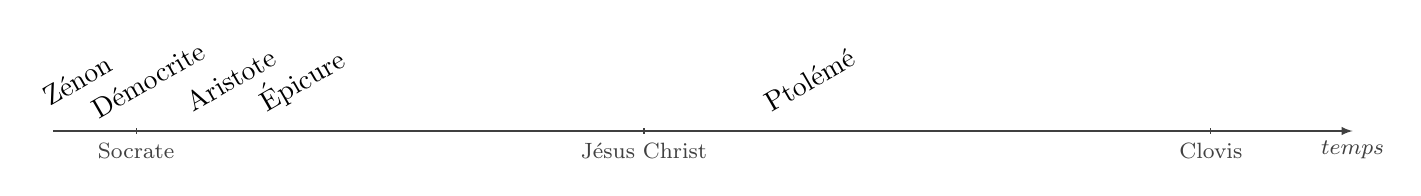
\begin{tikzpicture}
    \def\horizontal {1.5}
    \def\vertical {1.3}
\draw[-latex,color=darkgray] (-5*\horizontal,0) -- (6*\horizontal,0);
\draw[shift={(6*\horizontal,0)},color=darkgray,thin]
                                   node[below] {\footnotesize $temps$};
%470-399 av JC
  \draw[shift={(-4.3*\horizontal,0)},color=darkgray,thin] (0pt,1pt) -- (0pt,-1pt)
                                   node[below] {\footnotesize Socrate};
  \draw[shift={(0,0)},color=darkgray,thin] (0pt,1pt) -- (0pt,-1pt)
                                   node[below] {\footnotesize Jésus Christ};
  \draw[shift={(4.8*\horizontal,0)},color=darkgray,thin] (0pt,1pt) -- (0pt,-1pt)
                                   node[below] {\footnotesize Clovis};
%490-430 av JC
\draw (-4.8*\horizontal,0.5*\vertical) node [rotate=30]{Zénon};
%460-370 av JC
\draw (-4.2*\horizontal,0.5*\vertical) node [rotate=30]{Démocrite};
%384-322 av JC
\draw (-3.5*\horizontal,0.5*\vertical) node [rotate=30]{Aristote};
%340-270 av JC
\draw (-2.9*\horizontal,0.5*\vertical) node [rotate=30]{Épicure};
%100-168%
\draw (1.4*\horizontal,0.5*\vertical) node [rotate=30]{Ptolémé};
\end{tikzpicture}

%
\subsection{Présocratique}

Zénon soutenait plusieurs paradoxe dont les plus fameux concernent le mouvement : un mobile ne peut atteindre le terme de son mouvement car pour cela il devrait parcourir la moitié du trajet, puis la moitié de la moitié restante, et ainsi de suite à l'infini. Selon Aristote, il est l'inventeur de la dialectique.

Démocrite admet la composition atomique de la matière, déterminé par le seul principe de causalité. Il préfigure la pensée scientifique, ainsi que celle d'épicure, de Lucrèce et de Descartes.

\subsection{Aristote}
Il dénonce comme faux les arguments de Zénon parce qu'ils s'appuient sur une représentation du temps trompeuse (constitué d'une addition d'instant).

Selon lui, il existe deux mécaniques, une terrestre (imparfaite) et une celeste (parfaite).
\begin{center}
\setlength{\fboxsep}{3mm}
\fbox{
Le mouvement naturel est le cercle
}
\end{center}
Les astres ont une trajectoire circulaire, leur mouvement est parfait et immuable.
Les corps terrestre, imparfait, rejoignent leur nature. La pierre tombe pour rejoindre la terre, le feu monte pour rejoindre le ciel.
%
\subsection{Ptolémé}
%
Les astres errant parcourent des épicycles, expliquant ainsi les rétrogradations observées.
%
%%%%%%%%%%%%%%%%%%%%%%%%%%%%%%%%%%%%%%%%%%%%%%%%%%%%%%%%%%%%%%%%%%%%%%%%%%%%%%%%%%%%%
